\documentclass[11pt, a4paper]{article}

\usepackage{graphicx}
\usepackage[english]{babel}
\usepackage[utf8x]{inputenc}
\usepackage{amsmath}
\usepackage[a4paper,top=3cm,bottom=2cm,left=2cm,right=2cm,marginparwidth=1.75cm]{geometry}
\usepackage{amssymb}

\graphicspath{ {./images} }

\makeatletter
\renewcommand*\env@matrix[1][*\c@MaxMatrixCols c]{%
  \hskip -\arraycolsep
  \let\@ifnextchar\new@ifnextchar
  \array{#1}}
\makeatother

\begin{document}

\setcounter{section}{2}
\section{Lecture 3: Matrix-vector products and solution sets (18/02/2020)}

\subsection{general form of vectors and matrices}
Matrices can be thought of an $m \times n$ grid of numbers. A column vector is thus by extension
of the form $1 \times n$. let the $\vec{x}$ be a random column vector and $A$ a $m \times 1$ matrix.  
Then: 
\begin{align*}
  A = 
  \begin{bmatrix}[cccc]
    a_1 & a_2 & \cdots & a_m\\
  \end{bmatrix}
  \quad \text{and} \quad 
  \vec{x} = 
  \begin{bmatrix}
    x_1\\
    x_2\\
    \vdots \\
    x_n\\
  \end{bmatrix}
\end{align*}
\\
The matrix vector product is defined as the following:

\begin{align*}
  \vec{y} = A\vec{x} =
  \begin{pmatrix}
    a_{11}x_1 + \cdots + a_{1n}x_n\\
    a_{21}x_1 + \cdots + a_{2n}x_n\\
    \vdots\\
    a_{m1}x_1 + \cdots + a_{mn}x_n\\
  \end{pmatrix}
\end{align*}
\\
It is thus possible to compute the matrix-vector product using this definition, it's worth noting that
$A\vec{x}$ of the form $m \times n$ will always be of the form $\vec{x} \in \mathbb{R}^n$ and 
$\vec{y} = \mathbb{R}^m$. Which is to say, The matrix vector product of an $m \times n$ 
matrix and vector of $n$ entries will output
a vector with $m$ entries.\\
\\
A quick numerical example will follow:
\begin{align*}
  \begin{bmatrix}[cc]
    2 & 0\\
    3 & 2\\
    1 & 2\\
  \end{bmatrix}
  \cdot
  \begin{pmatrix}
    1\\
    3\\
  \end{pmatrix}
  =
  1 \cdot \begin{pmatrix} 2\\ 3\\ 1\\ \end{pmatrix} +
  3 \cdot \begin{pmatrix} 0\\ 2 \\ 2\\ \end{pmatrix} =
    \begin{pmatrix} 2+0\\ 3+6\\ 1+6\\ \end{pmatrix}
  =
  \begin{pmatrix} 1\\ 9\\ 7\\ \end{pmatrix}
\end{align*}

\subsection{Algebraic rules for matrix vector multiplication}
There are some important algebraic rules to note for matrix-vector multiplication. All properties
relating to manipulation of matrix-vector multiplication can be derrived using these 2 definitions.
let $A$ be an $m \times n$ matrix, $\vec{v}$ and $\vec{u}$ $1 \times n$ vectos and $c$ and $d$ a scalar.
\begin{gather}
  A(\vec{u} + \vec{v}) = A\vec{u} + A\vec{v}\\
  A(c\vec{u}) = c(A\vec{u})
\end{gather}
Combining equation (1) and (2) gives the following, which is also sometimes given as a third rule:
\begin{gather}
  A(c\vec{u} + d\vec{v}) = c(A\vec{u}) + d(A\vec{v})
\end{gather}

It's worth noting that matrix-multiplication can alternetivly be interpreted as the dot product
between a row in the matrix and the column vector $\vec{v}$. Thinking about it this way can save time
when computing matrix-vector products.

\subsection{Notations for matrix-vector products}
All the following forms are equavalant: 
\begin{align*}
  \begin{cases}
    x + 2y + 3z =3\\
    2x - y -2z = 4\\
    -x + y + 3z = 5\\
  \end{cases}
  \Leftrightarrow
  x \cdot \begin{pmatrix} 1\\ 2\\ -1\\ \end{pmatrix} +
    y \cdot \begin{pmatrix} 2\\ -1\\ 1\\ \end{pmatrix} +
    z \cdot \begin{pmatrix} 3\\ -2\\ 3\\ \end{pmatrix} =
    \begin{pmatrix} 3\\ 4\\ -5\\ \end{pmatrix}
  \Leftrightarrow
  \begin{bmatrix}
    1 & 2 & 3\\
    2 & -1 & -2\\
    -1 & 1 & 3\\
  \end{bmatrix}
  \cdot
  \begin{pmatrix} x\\ y\\ z\\ \end{pmatrix}
  =
  \begin{pmatrix} 3\\ 4\\ -5\\ \end{pmatrix}
\end{align*}

\subsection{Homogenous and Non-homogenous systems}
Is system is defined to be homogenous if $A\vec{x} = \vec{y}$ where $\vec{y} = 0$.
Conversly a system is defined to be non-homogenous if $A\vec{x} = \vec{y}$ where $\vec{y} \neq 0$.
Homogenous systems have some interesting properties. These are as follows:
\begin{itemize}
  \item Homogenous systems are always consistent, and thus always have a solution
  \item Homogenous systems have a non-trivial\footnote{a trvial solution is a solution where all variables are 0. It's technically true but doesn't tell us anything about the system.} 
        solution if and only if it has 1 free variable.
\end{itemize}

Some examples of homogenous and non-homogenous systems will follow:
\begin{align*}
  \begin{bmatrix}[ccc|c]
    3 & 4 & -5 & 0\\
    -3 & -2 & 1 & 0\\
    6 & 1 & 4 & 0\\
  \end{bmatrix}
  \sim
  \begin{bmatrix}
    1 & 0 & 1 & 0\\
    0 & 1 & -2 & 0\\
    0 & 0 & 0 & 0\\
  \end{bmatrix}
  \Rightarrow
  \begin{pmatrix} x_1 \\ x_2 \\ x_3 \end{pmatrix}
  = \begin{pmatrix} -x_3\\ 2x_3\\ x_3\\ \end{pmatrix}
  = x_3 \cdot \begin{pmatrix} -1\\ 2\\ 1\\ \end{pmatrix}
\end{align*}

\begin{align*}
  \begin{bmatrix}[ccc|c]
    3 & 4 & -5 & 1\\
    -3 & -2 & 1 & 1\\
    6 & 1 & 4 & -5\\
  \end{bmatrix}
  \sim
  \begin{bmatrix}
    1 & 0 & 1 & -1\\
    0 & 1 & -2 & 1\\
    0 & 0 & 0 & 0\\
  \end{bmatrix}
  \Rightarrow
  \begin{pmatrix} x_1 \\ x_2 \\ x_3 \end{pmatrix}
  = \begin{pmatrix} -1 - x_3\\ 1 + 2x_3\\ x_3\\ \end{pmatrix}
  = \begin{pmatrix} -1\\ 1\\ 0\\ \end{pmatrix} + x_3 \cdot \begin{pmatrix} -1\\ 2\\ 1\\ \end{pmatrix}
\end{align*}
\\
Note that the part depending on the free variable does not change between homogenous 
and non-homogenous systems. Graphically this ca be interpreted as shifting the line of 
infinite solutions away  from the origin by some vector (illustrated in figure 1). For this example that vector is 
$\langle -1, 1, 0 \rangle$. Because of this general solution to a non-homogenous system can
be written in the form  $\vec{x} = \vec{x}_p + \vec{x}_h$., where $\vec{x}_p$ is the particular
solution and $\vec{x}_h$ the homogenous solution\footnote{This looks very similar to the solution of a 
non-homogenous differential equation (Analyse 1)}. 
It can be proven that these are any and all solutions to the system. (maybe insert proof later idk yet)

\begin{figure}[h]
  \centerline{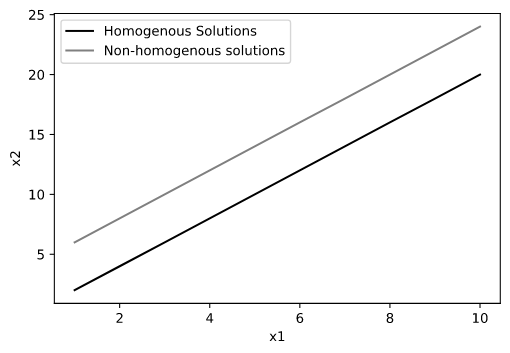
\includegraphics[width=10cm]{images/Solution_sets.png}}
  \caption{Comparison between the solution sets $\vec{v}_1 = 2\vec{v}_2$ and $\vec{v}_1 = 2\vec{v}_2 + \langle 0, 4 \rangle$.4
  Note that the second solution set is offset from the origin by the vector $\vec{b} = \langle 0, 4 \rangle$}
\end{figure}

\end{document}